\chapter{Considerações finais}
\label{consideracoes-finais}


\section{Resultados Prelimirares}
\label{results}

A partir da pesquisa realizada e do processo iniciado neste trabalho
\subsection{Plugins}

O \textit{plugin} que faz comunicação com o Ldap da UnB encontra-se em fase de homolagação
Com o auxilio de uma ferramenta de análise de código para \textit{Ruby} chamada Rcov, foi obtida a taxa de cobertura de código do plugin desenvolvido, além de alguns dados sobre a execução dos testes funcionais e unitários que seguem abaixo:

\begin{itemize}
\item Quantidade de testes executados: \textbf{96 testes;}
\item Quantidade de assertivas executadas: \textbf{111 assertivas;}
\item Quantiadde de falhas obtidas: \textbf{0 falhas;}
\item Tempo de execução dos testes: \textbf{7.8 segundos;}
\end{itemize}

Na imagem abaixo existem dois gráficos de cobertura de codigo, o primeiro definido como \textit{'total coverage'} representa a contagem realizada com as linhas em branco e os comentários do código, já o \textit{'code coverage'} representa a contagem realizada sem as linhas em branco e os comentários do código.

%
\begin{figure}[!h]
    \centering
    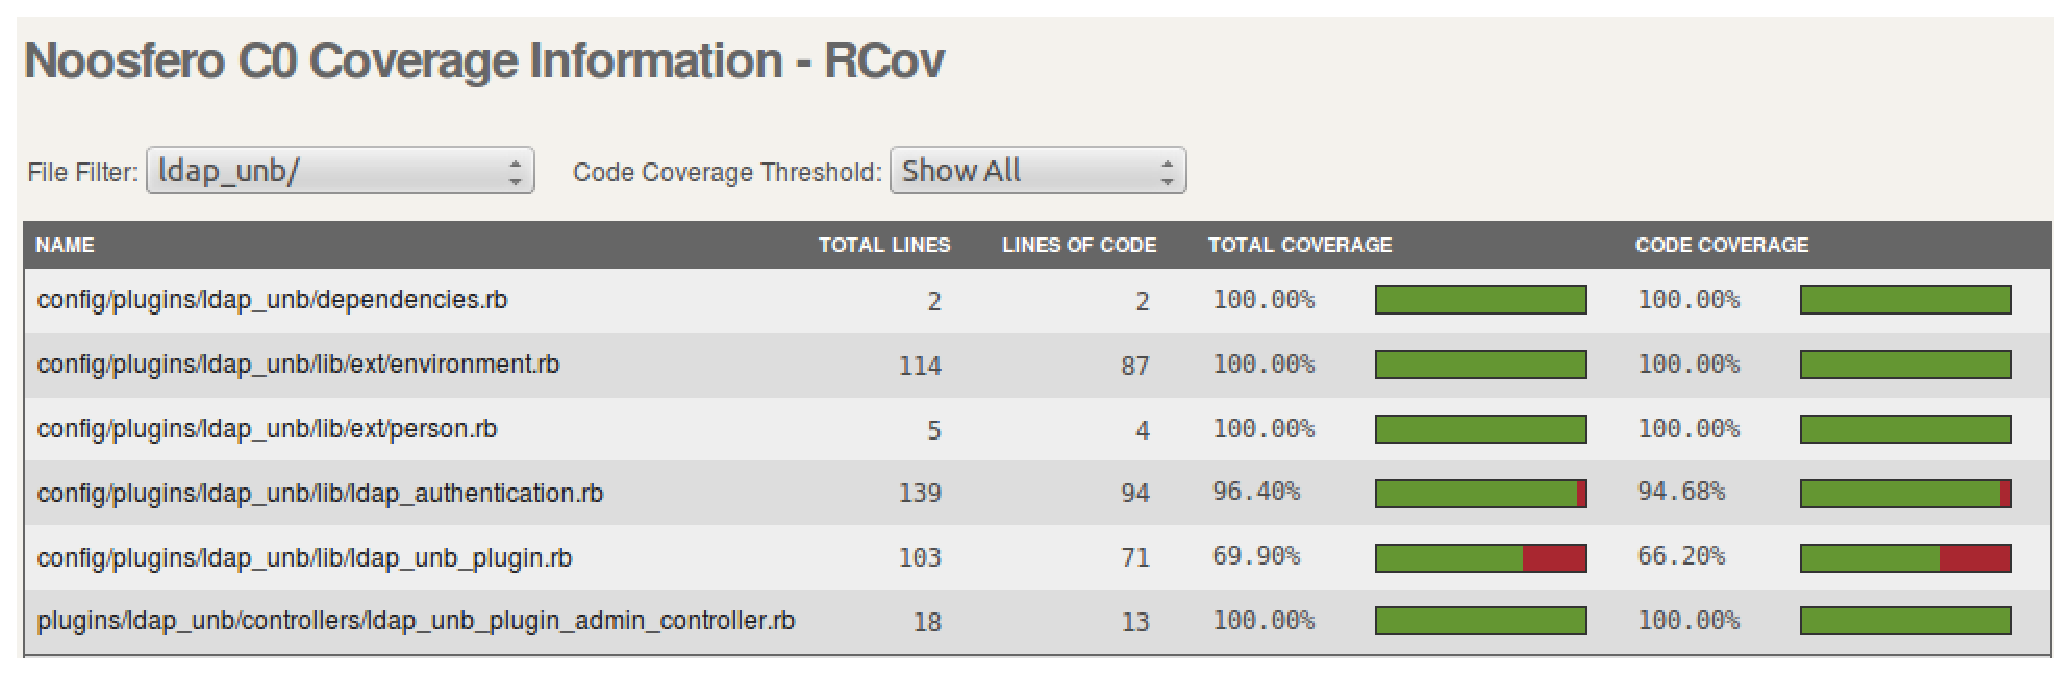
\includegraphics[keepaspectratio=false,scale=0.45]
      {figuras/cobertura_teste.eps}
    \caption{Cobertura de código do Plugin LdapUnb}
    \label{consideracoes_cobertura1}
\end{figure}
%


A ferramenta Rcov também foi utilizada para dimensionar a taxa de cobertura de código do plugin para envio de TCC, segue os dados sobre a execução dos testes funcionais e unitários:
\begin{itemize}
\item Quantidade de testes executados: \textbf{28 testes};
\item Quantidade de assertivas executadas: \textbf{84 assertivas};
\item Quantiadde de falhas obtidas: \textbf{0 falhas};
\item Tempo de execução dos testes: \textbf{10,5 segundos};
\end{itemize}

Na imagem abaixo está representado a cobertura de código, extraída da ferramenta Rcov:

\begin{figure}[!h]
    \centering
    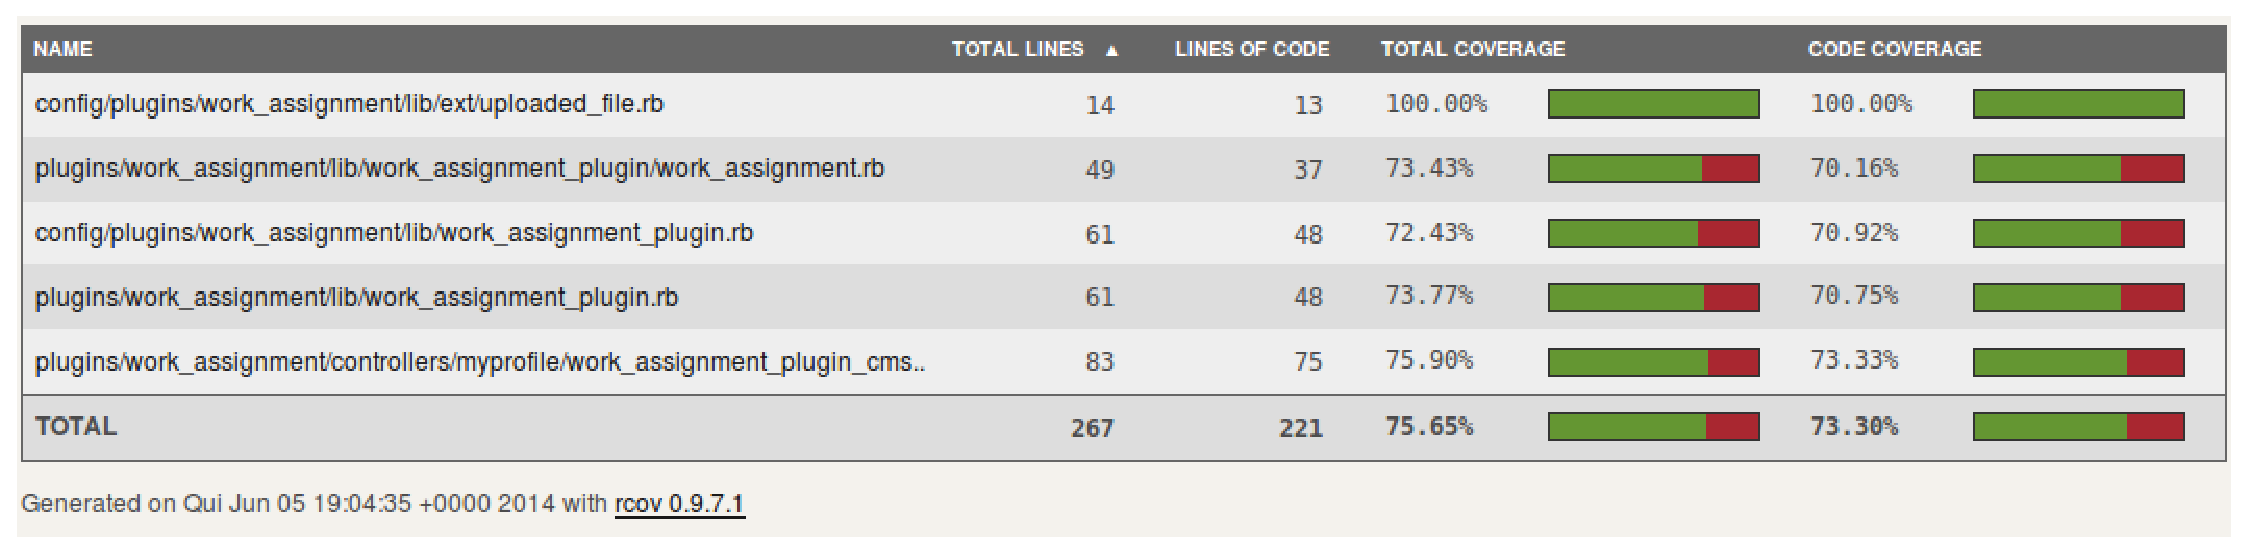
\includegraphics[keepaspectratio=false,scale=0.45]
      {figuras/cobertura_tcc.eps}
    \caption{Cobertura de código do Plugin para envio de TCC}
    \label{consideracoes_cobertura2}
\end{figure}

Para este plugin também foram desenvolvidos testes automáticos de aceitação, afim de validar a experiência do usuário em diferentes cenários possiveis:
\begin{itemize}
\item Quantidade de cenários executados: \textbf{6 cenários};
\item Quantidade de passos executadas: \textbf{130 passos};
\item Quantiadde de falhas obtidas: \textbf{0 falhas};
\item Tempo de execução dos testes: \textbf{7 minutos e 18 segundos};
\end{itemize}

A partir da cobertura dos testes do plugin de envio de TCC, foi verificado que existe uma necessidade de refatoração desta funcionalidade, considerando alguns aspectos que dificultaram o desenvolvimento de testes desta funcionalidade, como a duplicação de código.

Porém estes resultados preliminares foram considerados satisfatórios, considerando que outros plugins desenvolvidos pela comunidade do Noosfero e já homolagados apresentam métricas semelhantes.
\begin{itemize}
\item Plugin Stoa: Plugin que inclui funcionalidades ao Stoa, rede colaborativa da USP (Universidade de São Paulo)

\begin{figure}[!h]
    \centering
    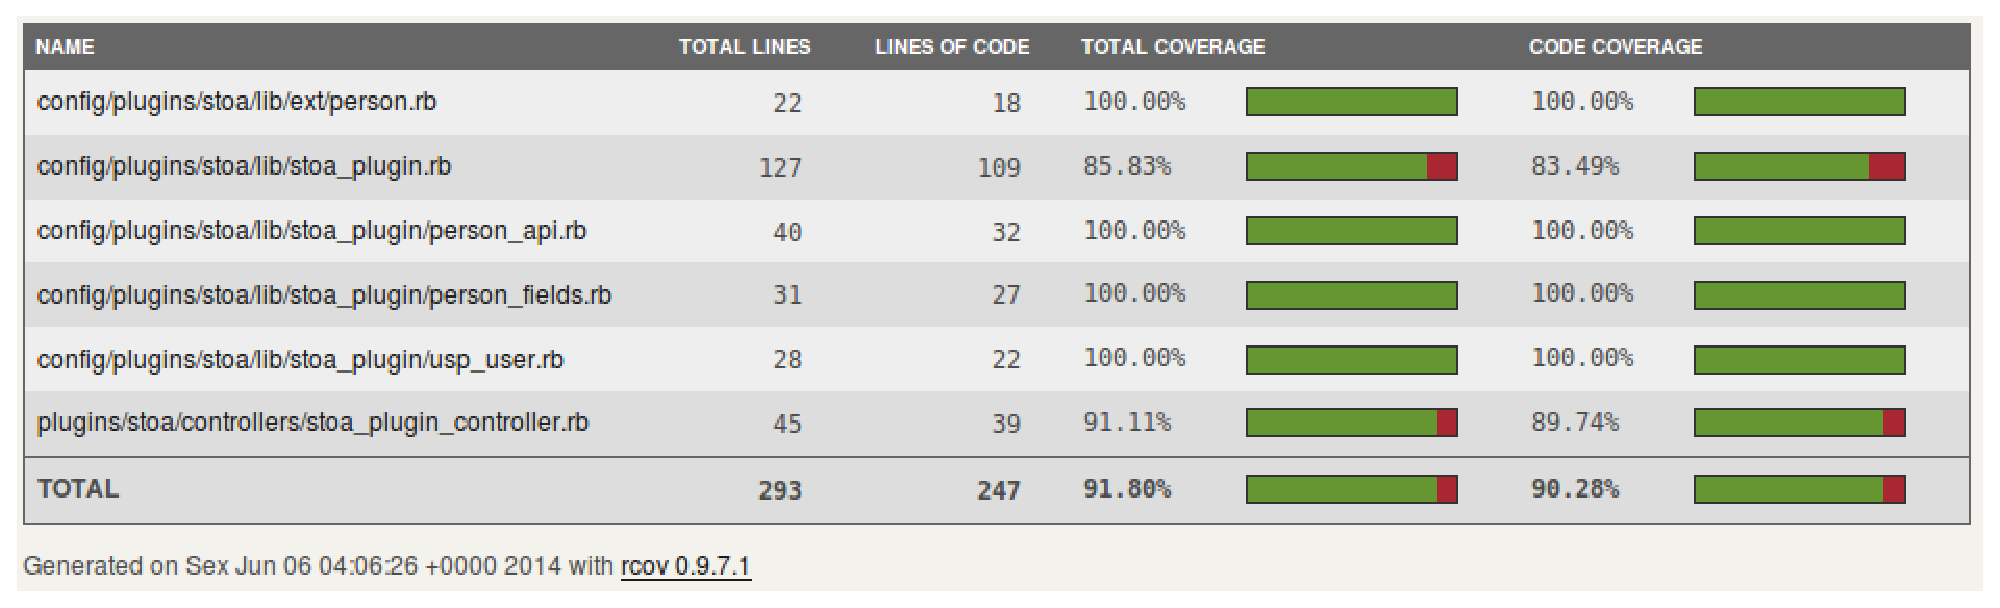
\includegraphics[keepaspectratio=false,scale=0.45]
      {figuras/stoa.eps}
    \caption{Cobertura de código do Plugin Stoa}
    \label{consideracoes_cobertura3}
\end{figure}

\item Plugin Ldap: Plugin que permite autenticação via Ldap;

\begin{figure}[!h]
    \centering
    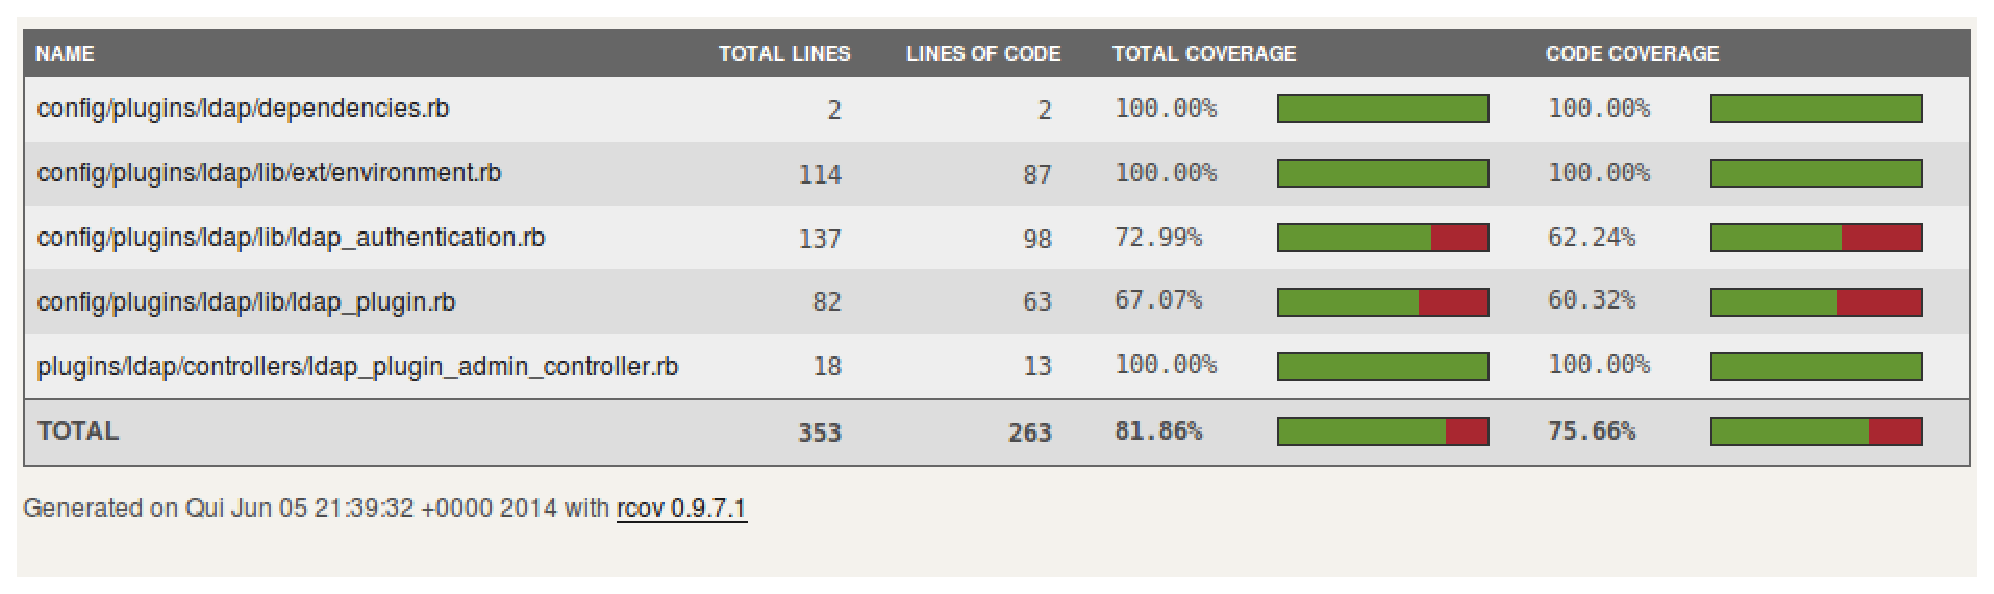
\includegraphics[keepaspectratio=false,scale=0.45]
      {figuras/ldap.eps}
    \caption{Cobertura de código do Plugin Ldap}
    \label{consideracoes_cobertura4}
\end{figure}

\item plugin Statistics: Plugin que permite adicionar um bloco de estatísticas ao perfil do usuário

\begin{figure}[!h]
    \centering
    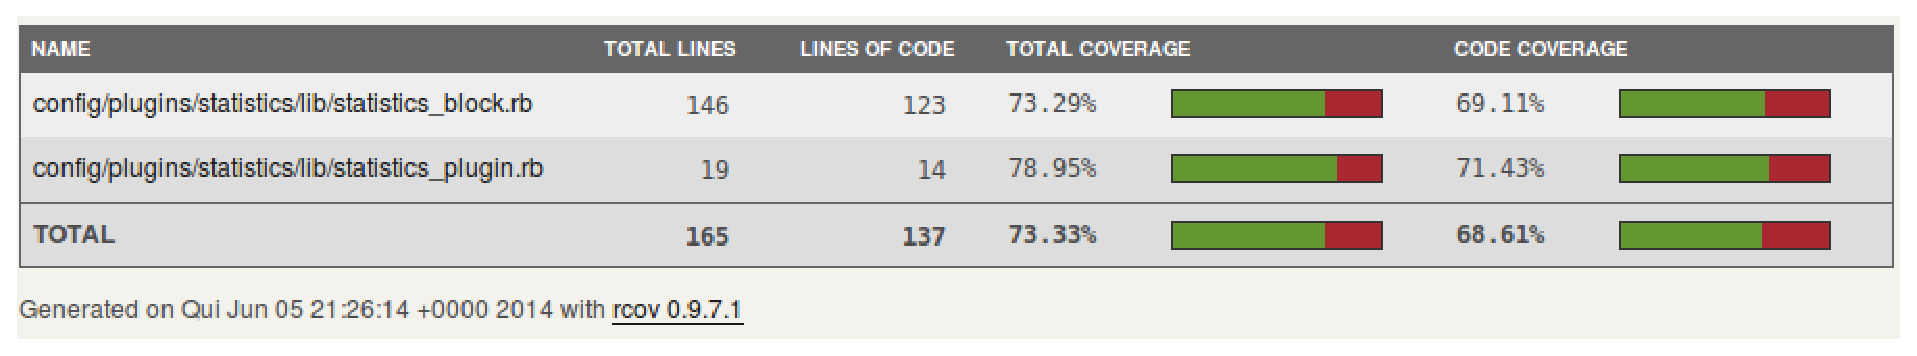
\includegraphics[keepaspectratio=false,scale=0.45]
      {figuras/statistics.eps}
    \caption{Cobertura de código do Plugin Statistics}
    \label{consideracoes_cobertura3}
\end{figure}

\end{itemize}

\section{Usabilidade no desenvolvimento de software empírico}

Com as pesquisas realizadas podemos notar que existe estudos na área onde foram criadas metodologias que unem tanto as abordagem ágeis com a abordagem centrada no usuário.

De acordo com os autores pesquisados é possível fazer a integração das abordagens, mas é necessário que tenha algumas adaptações.

% escrever detalhes

\section{Portal da Participação Social} 

	A ideia do estudo de caso proposto era conhecer como funciona algumas técnicas de avaliação da usabilidade. Foi escolhido o Portal da Participação Social por ser um dos projetos apoiado pela faculdade.

	Primeiramente precisou conhecer quem são os usuários do portal e quais são seus interesses. Para isso foi proposto algumas técnicas para análise do perfil do usuário: como aplicação de questionário de perfil de uso, análise de dados estatísticos e criação de persona do usuário.

	A Persona foi criada analisando alguns usuários cadastrados no portal e através de informações tanto no perfil do portal, como de informações em redes sociais e sites pessoais conseguimos captar algumas informações de um determinado público do site.

	Com a persona identificada é possível criar alguns cenários de uso do sistema, na qual as tarefas levantadas farão parte do teste de usabilidade.

	Antes de realizar o teste de usabilidade com o usuário é importante que sejam verificadas as tarefas que serão executadas pelos participantes.Essas tarefas podem ser encontradas através da avaliação por heurísticas de usabilidade onde podemos descobrir antecipadamente os principais problemas na interface do sistema.

	Para analisar o grau de satisfação do usuário foi feito uma pesquisa com os principais questionários existentes e escolhemos o PSSUQ por acharmos que era o questionário que possuia maior grau de confiabilidade e que retornava quatra fatores (Satisfação Geral, Qualidade da Interface, qualidade da informação e utilidade do sistema).

	Também foi escolhido o questionário ASQ que é aplicado depois de cada tarefa executada. Além disso ao aplicar o teste de usabilidade é preciso observar atentamente os passos que os usuário está realizando para concluir cada tarefa.


\section{Próximos Passos}

Nesta seção está descrita suscitamente a proposta dos próximos passos deste trabalho de conclusão de curso. Basicamente, buscamos aplicar as técnicas de usabilidade pesquisadas durante o trabalho, em um processo baseado em BDD e TDD, a fim de verificar problemas de usabilidade, e satisfação e uso em um estudo de caso específico, no caso plataforma Noosfero. 

Outro passo a ser realizdo é verificar os padrões de design e usabilidade adotados pelo Noosfero e propor possíveis melhorias.

\subsection{Portal do Software Público}

Criado em 12 de abril de 2007, o portal do SPB já conta com mais de 60 soluções voltadas para diversos setores. Para a SLTI, o portal já se consolidou como um ambiente de compartilhamento de softwares. Isso resulta em uma gestão de recursos e gastos de informática mais racionalizada, ampliação de parcerias e reforço da política de software livre no setor público~\footnote{www.softwarepublico.gov.br}. 

As tecnologias de informação e comunicação estão se consolidando como meios de expressão do conhecimento, de expressão cultural e de transações econômicas. Na sociedade em rede, baseada em comunicação feita através de computadores, não é possível aceitar que as linguagens usadas nessa comunicação fiquem sob o poder de apenas alguns gigantes. No desenvolvimento de software que apresenta código aberto, como o SPB, as inovações são compartilhadas entre todos, permitindo que as melhorias sejam adotadas por qualquer um, assim o conhecimento passa a ser sempre disseminado, ajudando principalmente as pequenas e médias empresas~\footnote{www.softwarepublico.gov.br}.

A evolução do software publico ja passou por tres etapas de desenvolvimento e está na sua quarta etapa, contando com seus usuários para desenvolver novas funcionalidades e melhorias, a partir de sugestões dadas pelos mesmos.

o portal foi desenvolvido baseado na plataforma Noosfero, e a partir disso planejamos aplicar no Portal os estudos que foram desenvolvidos neste trabalho, a avaliação de usabilidade a partir do desenvolvimento baseado em testes automatizados, a fim de responder se o processo de desenvolvimento utilizando práticas do BDD e TDD apresentam melhores resultados em testes de usabilidade.

\subsection{Cronograma}
